\begin{figure}[h]
    \centering
    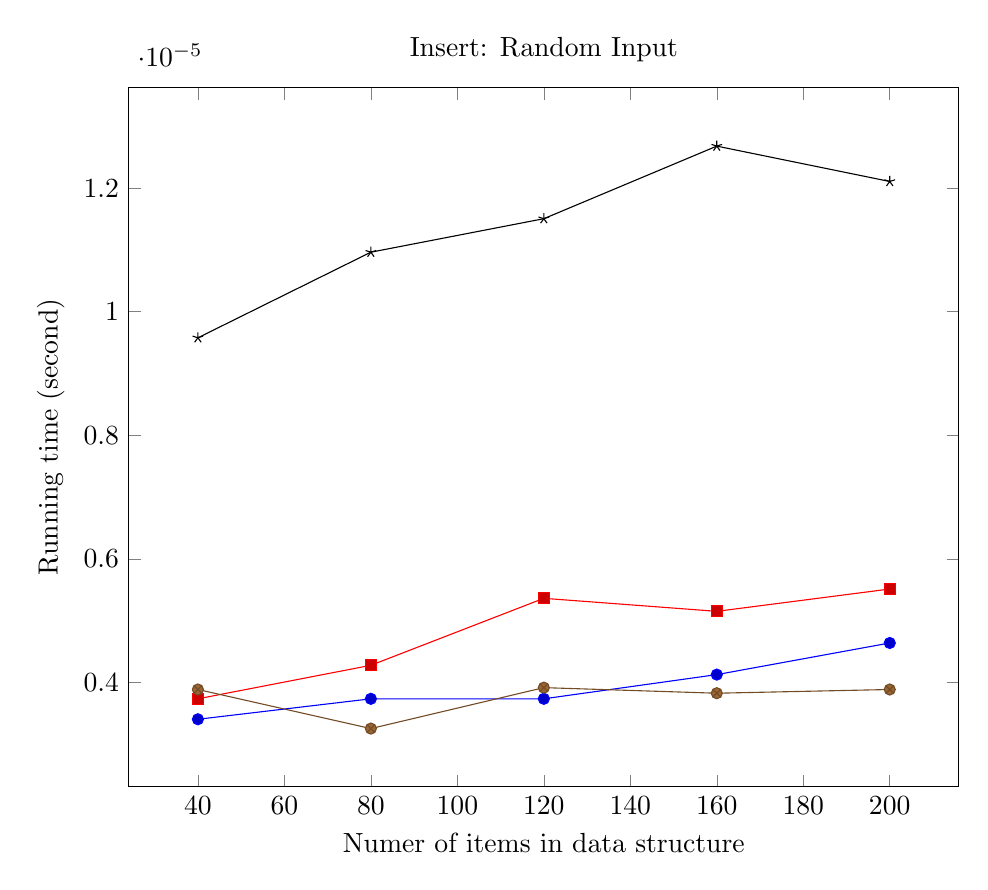
\begin{tikzpicture}
        \begin{axis}[
            xlabel={Numer of items in data structure},
            ylabel={Running time (second)},
            title={Insert: Random Input},
            width=\textwidth
        ]
		\addplot coordinates {
			(200, 4.6381001859757e-06)
			(160, 4.1261021134976485e-06)
			(120, 3.7345741757208867e-06)
			(80, 3.7345741757208867e-06)
			(40, 3.403281305293729e-06)
		};
		\addplot coordinates {
			(200, 5.511508662555883e-06)
			(160, 5.1500982584534035e-06)
			(120, 5.360920994179619e-06)
			(80, 4.276689781873913e-06)
			(40, 3.7345741757208867e-06)
		};
		\addplot coordinates {
			(200, 3.885161844096457e-06)
			(160, 3.82492677674616e-06)
			(120, 3.91527937777178e-06)
			(80, 3.252693636918158e-06)
			(40, 3.885161844096457e-06)
		};
		\addplot coordinates {
			(200, 1.2107248537417126e-05)
			(160, 1.2679481677245475e-05)
			(120, 1.1504897863914149e-05)
			(80, 1.0962782257761122e-05)
			(40, 9.577375708703233e-06)
		};
        \legend{}
        \end{axis}
    \end{tikzpicture}
    \caption{Average of 0 operations, benchmarked every 0, starting at 0.}
\end{figure}